%
% $RCSfile: data_mapper.tex,v $
%
% Copyright (C) 2002-2008. Christian Heller.
%
% Permission is granted to copy, distribute and/or modify this document
% under the terms of the GNU Free Documentation License, Version 1.1 or
% any later version published by the Free Software Foundation; with no
% Invariant Sections, with no Front-Cover Texts and with no Back-Cover
% Texts. A copy of the license is included in the section entitled
% "GNU Free Documentation License".
%
% http://www.cybop.net
% - Cybernetics Oriented Programming -
%
% http://www.resmedicinae.org
% - Information in Medicine -
%
% Version: $Revision: 1.1 $ $Date: 2008-08-19 20:41:06 $ $Author: christian $
% Authors: Christian Heller <christian.heller@tuxtax.de>
%

\subsubsection{Data Mapper}
\label{data_mapper_heading}
\index{Data Mapper Pattern}
\index{Data Source Layer}
\index{Database Layer}
\index{Entity Relationship Model}
\index{ERM}
\index{Data Mapper Layer}
\index{Domain Model Layer}
\index{Persistence Model Layer}
\index{Object Finder Interface}
\index{Object Mapper Implementation}
\index{Mediator Pattern}
\index{Bidirectional Dependencies in Data Mapper Pattern}
\index{Translator Architecture}

Besides the \emph{Domain Model}, figure \ref{logical_figure} contained a layer
called \emph{Data Source} which may for example represent a database. Normally,
both layers need to exchange data. Modern systems use OOP methods to implement
the domain model. Database models, on the other hand, are often implemented on
the basis of an \emph{Entity Relationship Model} (ERM). In order to avoid close
coupling and a mix-up of both layers, the introduction of an additional
\emph{Data Mapper} layer \cite{fowler2002} in between the two others may be
justified (figure \ref{datamapper_figure}). The most important idea of this
pattern is to abolish the interdependencies of domain- and persistence model
(database).

\begin{figure}[ht]
    \begin{center}
        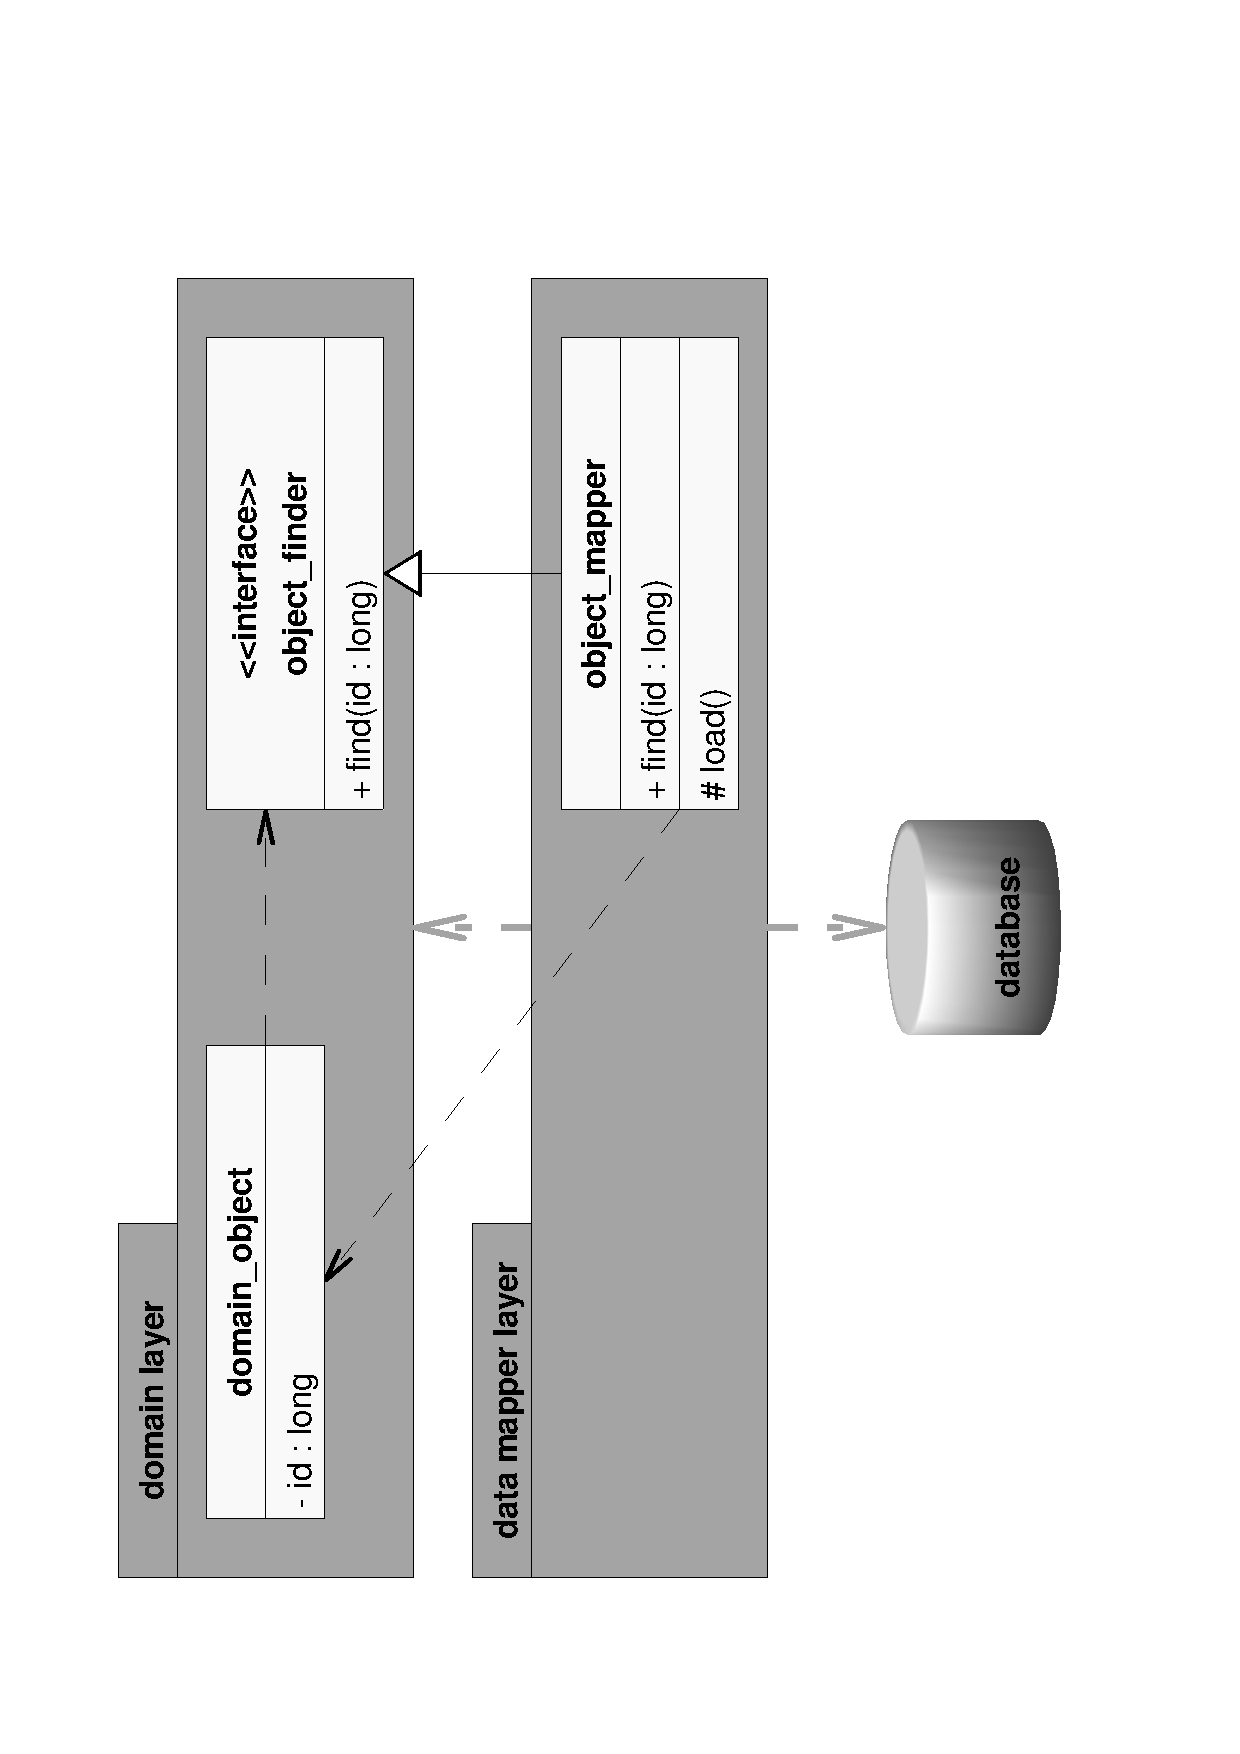
\includegraphics[scale=0.3,angle=-90]{graphic/datamapper.pdf}
        \caption{Data Mapper Pattern}
        \label{datamapper_figure}
    \end{center}
\end{figure}

The dashed arrows in figure \ref{datamapper_figure} indicate dependencies. The
data mapper layer knows the domain model- as well as the data source layer, via
\emph{unidirectional} relations. Its task is to \emph{translate} between the
two, in both directions. Domain model and data source know nothing from each
other. Each domain model class knows its appropriate \emph{object\_finder}
interface but does not know the implementation of the same. That is,
persistence- and data retrieval mechanisms are hidden in front of the domain
model. The \emph{object\_mapper} implementation is part of the mapping package
and also implements all finder methods. It maps data of the received result
sets to the special attributes of the domain model objects.

The \emph{Mediator} pattern \cite{gamma1995} is similar to the \emph{Mapper}, in
that it is used to decouple different parts of a system. Fowler \cite{fowler2002}
writes: \textit{\ldots\ the objects that use a mediator are aware of it, even if
they aren't aware of each other; the objects that a mapper separates aren't even
aware of the mapper.}

Although the \emph{Data Mapper} pattern is very helpful at implementing OO
systems, two things are to be criticised: Firstly, since the \emph{object\_finder}
relies on functionality specific to the retrieval of persistent data, it does
actually belong into the data mapper layer what, if done, would create
bidirectional dependencies between the domain model- and data mapper layer. But
also with the \emph{object\_finder} remaining in the domain model layer,
dependencies are not purely unidirectional. It is true that from an OO view,
they are. Internally, however, a super class or interface relates to its
inheriting classes, so that it can call their methods to satisfy the
polymorphic behaviour.

Secondly, the layers do not truly build on each other. Taken an architecture
similar to the one in figure \ref{logical_figure}, consisting of the following
five instead of only three layers:

\begin{enumerate}
    \item Presentation
    \item Application Process
    \item Domain Model
    \item Data Mapper
    \item Data Source
\end{enumerate}

\ldots\ the application process does not only access the domain model layer, it
also has to manage (create and destroy) the objects of the data mapper layer.
In other words, it surpasses (disregards) the domain model layer when accessing
the data mapper layer directly.

Chapter \ref{state_and_logic_heading} will describe how a strict separation of
state- and logic knowledge allows to access and translate runtime models
unidirectionally.
